\section{Potentialfeld zur Bahngenerierung und Kollisionsvermeidung}
\label{sec:Potential}
In diesem Abschnitt wird beschrieben, wie das Potentialfeld aufgebaut ist, dass zur Generierung des Geschwindigkeitsvektors genutzt wird.
\subsection{Roboter Umwelt}
Um die statische Umwelt des Robotinos im Potentialfeld darzustellen, wird der zu befahrende Bereich in Zonen unterteilt. Die gewählten Zonen sind in Abbildung \ref{fig:PotZonen} farbig dargestellt. In Tabelle \ref{tab:Zonen} ist die Zurordnung der Zonen zur Abbildung \ref{fig:PotZonen} beschrieben. Dabei wird eine Hauptfahrzone (Zone 0) definiert, in der mit einem virtuellen Zaun der zu befahrene Bereich abgegrenzt wird. Dieser Zaun ist notwendig, damit die Zone nicht unkontrolliert verlassen wird, dazu werden e-Funktionen genutzt, die wie in den Funktionen \ref{} bis \ref{} definiert sind. Aufgrund der Form der Zone müssen dabei drei Funktionen definiert werden, die je nach Position des Robotinos ausgeführt werden. Das Verlassen der Zone 0 erfolgt durch die Übergabe an den Fertigungsbereich, welches in Kapitel \ref{} näher erläutert wird. \\
Zone 1 bis 3 dienen zur Rückführung der Robotinos zur Zone 0, dazu wird ein Potentialfeld genutzt, dass uns ermöglicht den Robotino in eine geziehlte Richtung zu lenken. Die dazu genutzten Funktionen sind unter \ref{fun:H01} bis \ref{} definiert. Diese Potentialfelder nutzen in Fahrrichtung eine Geradengleichung mit definierter Steigung und senkrecht dazu eine Parabelform, um den Robotino auf Kurs zu halten. Wenn sich der Robotino in Zone 4 befindet, wird dieser über eine Geradengleichung noch hinten geführt. Die dbei genutzte Gleichung ist als \ref{} gekennzeichnet. Zusätzlich wird in Zone 4 für jede Station eine gaußsche radiale Basisfunktion, welche unter Kapitel \ref{} näher erläutert, genutzt, damit keine Kollision mit den Stationen auftreten. Diese Zone wird nur im Fehlerfall oder beim Start des Robotinos betreten, da in dieser Zone der Fertigungsbereich aktiv ist. Die Zone 5 dient dazu den Robotino geziehlt in Richtung der mitte der Zone 0 zu führen. Dazu wird wie in Zone 1 bis 3 eine Parabel- mit einer Geradengleichung genutzt. Die dabei genutzte Funktion ist als \ref{} definiert. Dabei ist zu beachten, dass vorgesehen ist, dass Zone 5 nur aktiv ist, wenn sie aus Zone 1 betreten wird. Dadurch wird die Anfahrmöglichkeit aus der Zone 0 zur Ladestation gewährleistet. \\
Je nach Zone gilt dabei ein eigenes Potentialfeld, welche kombiniert das Gesamtpotentialfeld ergebenen. Die einzelnen Zonen sind in Abbildung \ref{fig:Poteinzeln} dargestellt. Das gesamt Potentialfeld ist in Abbildung \ref{fig:PotUmweltohne} dargestellt, wobei zur Übersichtlichkeit die Stations und Ladestationspotentiale nicht dargestellt werden. Da die Zone 5 nur durchlaufen wird, wenn sie aus Zone 1 betreten wird, wird in Abbildung \ref{fig:PotUmweltmit} dargestellt, wie das Potentialfeld in diesem Fall aussieht.

\begin{table}
\centering
 \begin{tabular}{|c|c|c|}
  \hline Zone & Farbe & Beschreibung \\ 
  \hline 0 & ohne Farbe & Hauptfahrzone \\
  \hline 1 & Grün &  Führung des Robotinos nach Zone 5 \\
  \hline 2 & Blau &  Führung des Robotinos nach Zone 3 \\
  \hline 3 & Violet & Führung des Robotinos nach Zone 0 \\
  \hline 4 & Rot & Führung des Robotinos nach Zone 1 und 2\\
  \hline 5 & Cyan & Führung des Robotinos nach Zone 0 \\
   \hline \end{tabular}
   \label{tab:Zonen}
\end{table}

\begin{figure}
	\centering	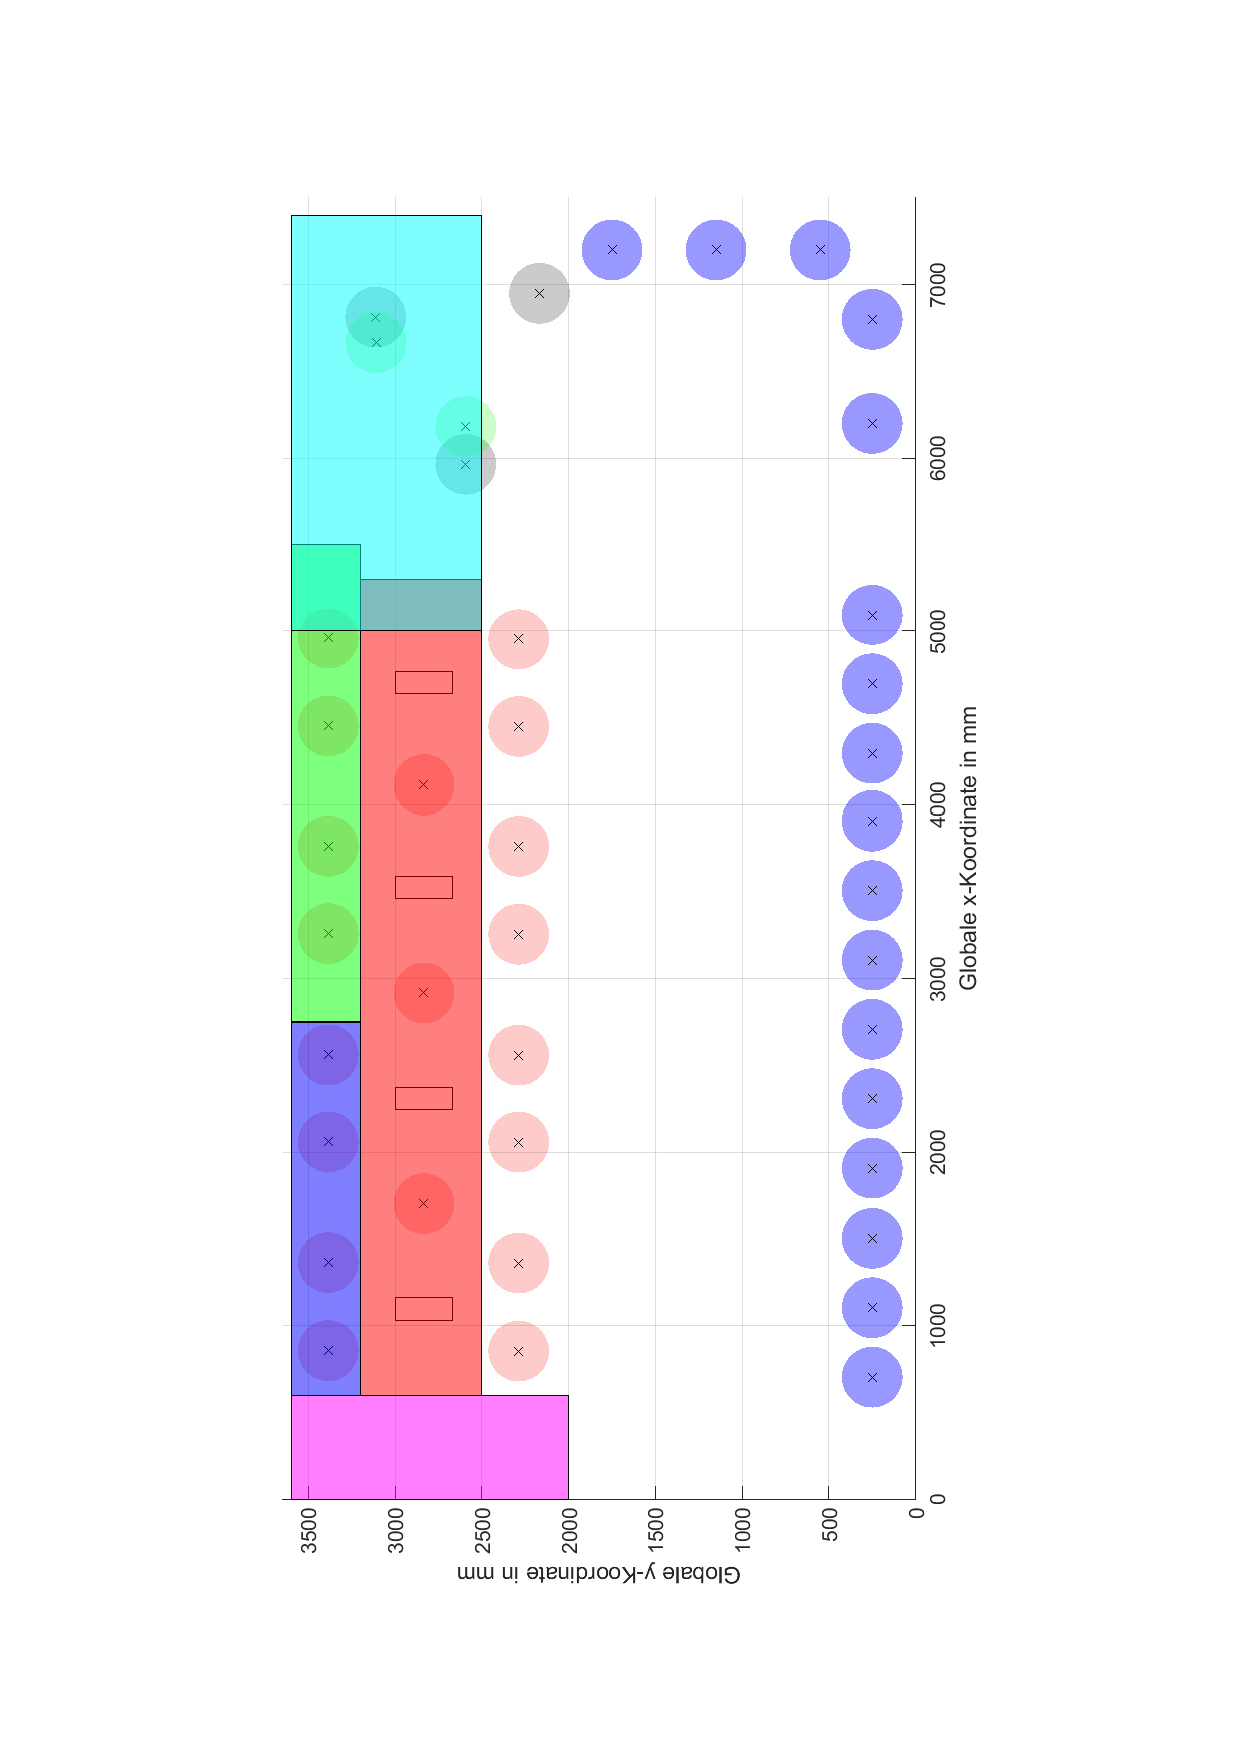
\includegraphics[width=0.8\textwidth, angle=-90]{grafiken/Zonen_eingezeichnet.pdf}
	\caption{Potentialfeldzonen}
	\label{fig:PotZonen}
\end{figure}

\begin{align}
H_{0(x=0..5500,y=0..2500)} = K_{exp}\cdot(e^{(-\frac{x}{\sigma})}+e^{(\frac{x-7400}{\sigma})}+e^{(-\frac{y}{\sigma})}+e^{(\frac{y-2500}{\sigma})} ) \label{fun:H01}\\ 
H_{0(x=5500..7400,y=0..2500)} = K_{exp}\cdot(e^{(-\frac{(x-5500)-(y-2500)}{\sigma})}+e^{(\frac{x-7400}{\sigma})}+e^{(-\frac{y}{\sigma})} )\\ 
H_{0(x=5500..7400,y=2500..3600)} = K_{exp}\cdot(e^{(-\frac{(x-5500)}{\sigma})}+e^{(\frac{(y-3600)}{\sigma})}+e^{(\frac{x-7400}{\sigma})}+e^{(-\frac{y}{\sigma})} )\\ 
H_{1} = - K_{gerade}\cdot x + K_{parabel}\cdot\frac{(y-3500)^2}{B}\\
H_{2} = K_{gerade}\cdot x + K_{parabel}\cdot\frac{(y-3500)^2}{B}\\
H_{3} = K_{parabel}\cdot\frac{(x-300)^2}{B} + K_{gerade}\cdot y\\
H_{4} = - K_{gerade}\cdot y\\
H_{5} = K_{parabel}\cdot\frac{(x-5500)^2}{B}-K_{gerade}\cdot y
 \end{align}

\begin{figure}
	\centering	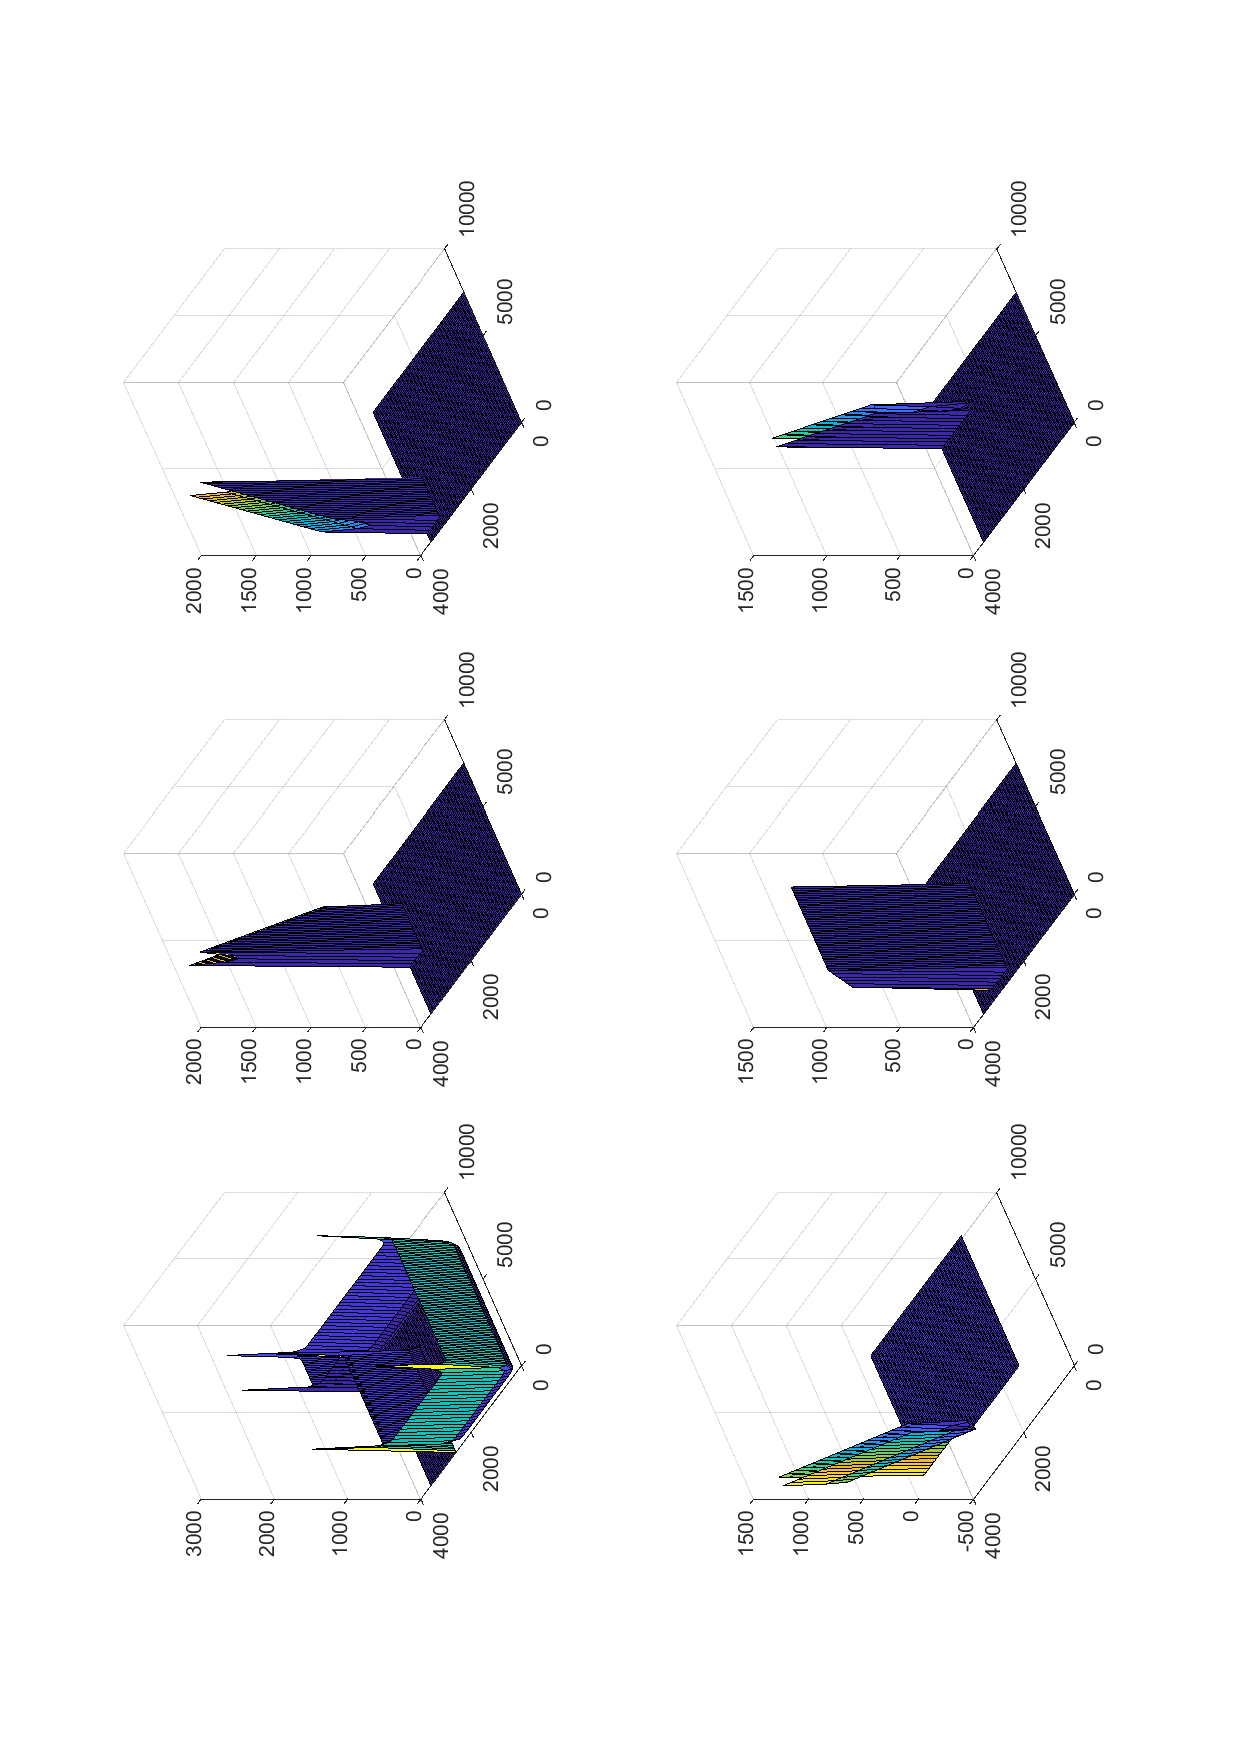
\includegraphics[width=0.5\textwidth,angle=-90]{grafiken/EinzelZonen.pdf}
	\caption{Potentialfeld der einzel Zonen}
	\label{fig:Poteinzeln}
\end{figure}

\begin{figure}
	\centering	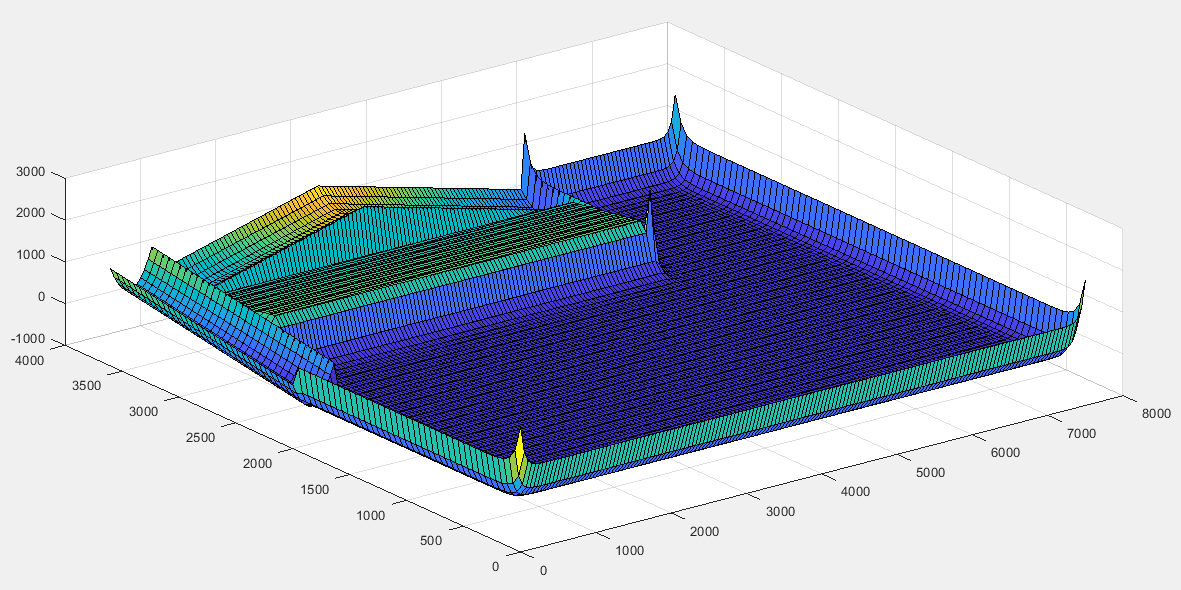
\includegraphics[width=0.5\textwidth]{grafiken/Potentialfeld_ohne_2schraege.png}
	\caption{Potentialfeld der Roboter Umwelt ohne Rausführung}
	\label{fig:PotUmweltohne}
\end{figure}

\begin{figure}
	\centering	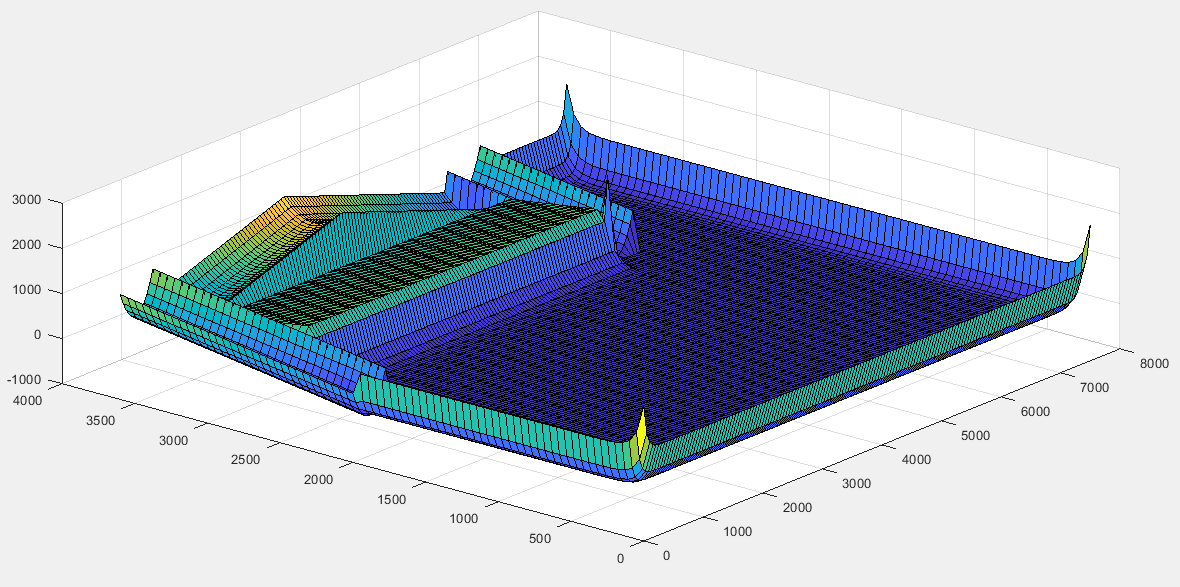
\includegraphics[width=0.5\textwidth]{grafiken/Potentialfeld_mit_2schraegen.png}
	\caption{Potentialfeld der Roboter Umwelt mit Rausführung}
	\label{fig:PotUmweltmit}
\end{figure}

\subsection{Robotino,Sationen und IR-Hindernisse}
Die Robotinos, die Stationen und die IR-Hindernisse werden im Potentialfeld als gaußsche radiale Basisfunktion betrachtet. Die genutzte Funktion ist unter \ref{} definiert. Da sich die gaußsche radiale Basisfunktion aufgrund der genutzten e-Funktion gut ableiten lässt, wird diese Funktion genutzt, um ein abstoßendes Potential zu generieren. Das Potentialfeld der gaußschen radialen Basisfunktion ist in Abbildung \ref{fig:PotRobotino} dargestellt. Dabei wird für die Stationen eine Konstante Position eingestellt. Die Position des Robotinos und der IR-Hindernisse werden als flexibel betrachtet, da sie während der laufzeit bestimmt werden müseen.. 

\begin{align}
H_{Gauß}=K\cdot e^{-\frac{(x-x_{pos})^2+(y-y_{pos})^2}{2\cdot \sigma^2}}
 \end{align}
 
\begin{figure}
	\centering	
\includegraphics[width=0.5\textwidth]{grafiken/listen-tiny.jpg}
	\caption{Potentialfeld der gaußschen radialen Basisfunktion}
	\label{fig:PotRobotino}
\end{figure}

\subsection{Ziel}
Das Ziel im Potentialfeld wird als Kegel mit konstantem Faktor realisiert. Dazu wird die in Gleichung \ref{} dargestellte Funktion genutzt. Um durch Trägheit verursachte Schwingungen um den Zielpunkt zu vermeiden, wird eine Abstandsabhängiger Faktor als Filterung nachgeschaltet. Dabei wird der Abstand über den Pythagoras bestimmt. Der dabei genutzte Faktor wird, wie in den Funktion \ref{} und \ref{} beschrieben, bestimmt. Das bei der Multiplikation von \(K_{Ziel} \cdot H_{Ziel} \) entstandene Potentialfeld ist in Abbildung \ref{fig:PotZiel} dargestellt.

\begin{align}
H_{Ziel}= K \cdot \sqrt{(x-x_{Ziel})^2+(y-y_{Ziel})^2} \\
K_{Ziel(Abstand_{ist} =< Abstand_{max}}=\frac{Abstand_{ist}}{Abstand_{max}}\\
K_{Ziel(Abstand_{ist} > Abstand_{max}}=1
 \end{align}
 
\begin{figure}
	\centering	
\includegraphics[width=0.5\textwidth]{grafiken/listen-tiny.jpg}
	\caption{Potentialfeld Ziel}
	\label{fig:PotZiel}
\end{figure}